\chapter{Mody Majorany jako lokalne całki ruchu}\label{chap:LIOMs}

\section*{Opis rozdziału}

W tym rozdziale zostanie przedstawiona metoda, która służy do identyfikacji operatorów \MZM, które są zachowane i lokalne. 
Algorytm został zaproponowany w naszej pracy~\cite{wieckowski.maska.2018}.

\section{Lokalne całki ruchu}

Schemat postępowania algorytmu, opisanego w tym rozdziale, jest bardzo podobny do metody wykorzystanej do badania lokalnych całek ruchu (\acrshort{LIOM}) w modelu Heisen-\linebreak berga~\cite{mierzejewski.prelovsek.2015,mierzejewski.prosen.2015}.
\acrshort{LIOM} są szczególnie istotne w fizyce lokalizacji wielu ciał (\acrshort{MBL}).
Zainteresowanego czytelnika tematyką \acrshort{LIOM} i \acrshort{MBL} odsyłam do literatury
\cite{serbyn.papic.2013,huse.nandkishore.2014,chandran.kim.2015,imbrie.ros.2017,mierzejewski.kozarzewski.2018}.

W pracy~\cite{wieckowski.maska.2018} opracowaliśmy metodę, która pozwala na znajdowanie zachowanych, \textit{lokalnych} operatorów $\Gammaii=\sum_i \alphaii_{i} \gammai$, z rzeczywistymi współczynnikami $\alphaii_{i}$.
Lokalność oznacza w~tym przypadku, że każdy operator $\gammai\in\majoranaBase$ związany jest fizycznie tylko i wyłącznie z jednym węzłem sieci.
Bardziej formalną dyskusję dotyczącą lokalności można znaleźć w rozdziale~\ref{chap:identification}, gdzie zaprezentowano wyniki z \cite{wieckowski.maska.2018}.
Przedstawiona poniższa metoda jest ogólna i może być wykorzystana do badania dowolnego hamiltonianu.
Rozważmy hamiltonian w diagonalnej bazie stanów własnych $\hatH = \sum_n \Energy_n \qstate n \qstatet n$.
W celu badania w jakim stopniu dany operator zachowany jest w czasie, przydatną konstrukcją jest średnia $\barGammaii$  po nieskończonym czasie z operatora\footnote{Dowód można znaleźć w~dodatku~\ref{chap:derivations}.} 
\begin{equation}
    \barGammaii = \lim_{\timeNormal\to\infty}\frac1{\timeNormal}\int\limits_0^{\timeNormal}\text d\timeNormal' \,\,\Gammaii(\timeNormal') =
    \sum_{\Energy_n=\Energy_m}\,\Gammaii_{nm}\,\,\,\qstate n\qstatet m,\label{eq:gammaAvg}
\end{equation}
gdzie $\Gammaii_{nm} = \qstatet n \Gammaii \qstate m$, a $\qstate n$, $\qstate m$ i $\Energy_n$, $\Energy_m$ to są stany i energie własne hamiltonianu $\hatH$.
Jeśli $\barGammaii = \Gammaii$ to wtedy taki operator jest całkowicie zachowany --- jest to całka ruchu.
Taki operator komutuje z hamiltonianem $[\hatH,\Gammaii]=0$.

\begin{figure}
    \centering
    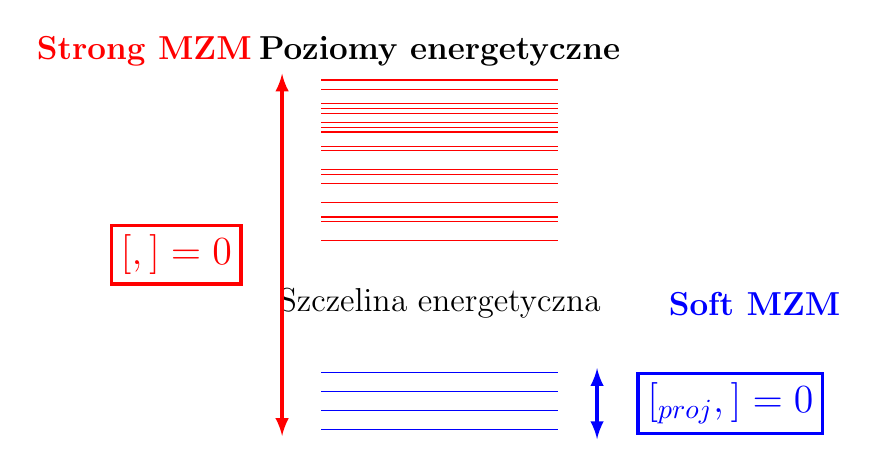
\begin{tikzpicture}[yscale=0.8]

\begin{scope}[blue,yscale = 1.5]
\draw (0,0) -- (3,0);
\draw (0,0.2) -- (3,0.2);
\draw (0,0.4) -- (3,0.4);
\draw (0,0.6) -- (3,0.6);
\draw [latex-latex,very thick] (3.5, -0.1) -- (3.5,0.65)node[midway,right,draw,very thick,xshift=0.5cm]{\Large
\colorlet{tmpcolor}{black}\colorlet{black}{blue}%
$[\hatH_\text{proj},\Gammaii] = 0$
\colorlet{black}{tmpcolor}%
};

\end{scope}


\begin{scope}[red,yscale = 1.5,yshift=2cm]
\draw (0,0) -- (3,0);
\draw (0,0.2) -- (3,0.2);
\draw (0,0.25) -- (3,0.25);
\draw (0,0.4) -- (3,0.4);
\draw (0,0.6) -- (3,0.6);
\draw (0,0.7) -- (3,0.7);
%\draw [white] (3.5, -0.1) -- (3.5,1.25)node[midway,right,draw,very thick,xshift=0.5cm,blue]{\Large $[\hatH,\Gammaii] \neq 0$};

\end{scope}
\begin{scope}[red,yscale = 1.5,yshift=2.75cm]
\draw (0,0) -- (3,0);
\draw (0,0.2) -- (3,0.2);
\draw (0,0.25) -- (3,0.25);
\draw (0,0.4) -- (3,0.4);
\draw (0,0.6) -- (3,0.6);
\draw (0,0.7) -- (3,0.7);
 
\end{scope}
\begin{scope}[red,yscale = 1.5,yshift=3.cm]
\draw (0,0) -- (3,0);
\draw (0,0.2) -- (3,0.2);
\draw (0,0.25) -- (3,0.25);
\draw (0,0.4) -- (3,0.4);
\draw (0,0.6) -- (3,0.6);
\draw (0,0.7) -- (3,0.7);
 
\end{scope}

\node[] at (1.5,2) {\large  Szczelina energetyczna};
\node[] at (1.5,6) {\bf \large Poziomy energetyczne};
\node[red] at (-2.25,6) {\bf \large Strong MZM};
\node[blue] at (5.5,2) {\bf \large Soft MZM};

\draw [latex-latex,very thick,red] (-0.5, -0.1) -- (-.5,5.65)node[midway,left,draw,very thick,xshift=-0.5cm]{
\colorlet{tmpcolor}{black}\colorlet{black}{red}%
\Large $[\hatH,\Gammaii] = 0$
\colorlet{black}{tmpcolor}%
};

\end{tikzpicture}
    \caption[Schematyczne porównanie strong i soft \textit{MZM}.]{Schematyczne porównanie strong i soft \MZM.}
    \label{fig:strongAndSoft}
\end{figure}

Omawiana w tym rozdziale metoda pozwala generować tzw. \textit{silne} \MZM\ (ang. \textit{strong}), które są stabilne dla dowolnie dużych temperatur~\cite{goldstein.chamon.2012,else.fendley.2017,kemp.yao.2017}.
\MZM\ $\Gammaii$, dla której warunek komutacji jest spełniony tylko i wyłącznie dla hamiltonianu $\hatH_{\text{proj}}$, który został zrzutowany do niskoenergetycznej podprzestrzeni  $[\hatH_{\text{proj}},\Gammaii]=0$, nazywamy \textit{słabą} \MZM\  (ang. \textit{soft})~\cite{alicea.fendley.2016}.
Na Rysunku~\ref{fig:strongAndSoft} schematycznie przedstawiono różnicę pomiędzy soft, a strong \MZM.


Poza specyficznymi wartościami parametrów układu, w skończonych układach \MZM\ nie są ściśle zachowane~\cite{kells.2015,sarma.freedman.2015}.
Relacja komutacji nie jest spełniona dokładnie
\begin{equation}
    [\hatH,\Gammaii] = \bigO(\eee^{-\sites/\corrLength}),\label{eq:nonzeroMZM}
\end{equation}
gdzie $\corrLength$ to długość związana z zanikaniem \MZM\ od brzegu układu, która zależy od parametrów hamiltonianu.
Niezerowa wartość komutatora \eqref{eq:nonzeroMZM} oznacza, że \MZM\ będzie miała skończony czas życia, a warunek komutacji \eqref{eq:MZMcom} będzie jedynie spełniony w granicy termodynamicznej.
Numerycznie można badać jedynie skończone układy, dlatego poszukiwanie operatorów \MZM\ można sprowadzić tylko i wyłącznie do problemu optymalizacyjnego współczynników $\alphaii_{i}$.

\ornament

\section{Korelacje wielociałowe}

Jako optymalny zestaw parametrów $\alphai$ rozumiemy taki zestaw, który 
generuje operatory $\barGammaii$ \textit{podobne} do $\Gammaii$ jak to tylko możliwe.
Jako kryterium podobieństwa operatorów wykorzystano iloczyn skalarny Hilberta--Schmidta 
\begin{equation}
    (A|B)=\Tr(A^\dagger B) / \Tr(\bbone).\label{eq:hilbertSchmidtInnerProductDef}
\end{equation}
Taki iloczyn skalarny odpowiada uśrednianiu termicznemu dla nieskończonych temperatur.
Jako kryterium podobieństwa można również wprowadzić odpowiedni iloczyn skalarny dla skończonych temperatur
\begin{equation}
    (A|B)_{\betaT} = \Tr(\eee^{-\betaT \hatH}A^\dagger B) / \Tr(\eee^{-\betaT \hatH}).
\end{equation}
W skończonych temperaturach czas życia \MZM\ jest większy.
W referencji \cite{mierzejewski.prosen.2015} można znaleźć inne propozycje iloczynu skalarnego.
Korzystając z iloczynu skalarnego można zdefiniować normę operatorów
\begin{equation}
    \| A \| = \sqrt{(A|A)} = \sqrt{\Tr(A^\dagger A)/\Tr(\bbone)}.
\end{equation}
Zadanie znalezienia najbardziej podobnego $\barGammaii$ do $\Gammaii$ sprowadza się do znalezienia współczynników $\alphai= (\gammai|\Gammaii)$, które będą minimalizowały następujący kwadrat normy\footnote{\label{footnote:normOpt}Dowód można znaleźć w~dodatku~\ref{chap:derivations}.}
\begin{equation}
    \|(\Gammaii-\barGammaii) \|^2 = 1 - \|\barGammaii\|^2.\label{eq:normOpt}
\end{equation}
Równość~\eqref{eq:normOpt} wynika z ważnej tożsamości\footref{footnote:normOpt} 
\begin{equation}
    (\barGammaii | \barGammaii) = (\barGammaii | \Gammaii) = (\Gammaii|\barGammaii).\label{eq:barGammabarGamma}
\end{equation}
W celu optymalizacji $\alphai$ należy zmaksymalizować $\|\barGammaii\|^2$
\begin{equation}
    \lambdai = \max_{\{\alphai\}}\|\barGammaii\|^2
    =\max_{\{\alphai\}}(\barGammaii|\barGammaii)
    = \max_{\{\alphai\}}(\barGammaii|\Gammaii) .\label{eq:lambdaDef1}
\end{equation}
Parametr $1-\lambdai$ mierzy odległość pomiędzy operatorami $\barGammaii$ i  $\Gammaii$.
W celu dalszej interpretacji parametru $\lambdai$ warto operator $\Gammaii$ rozłożyć w następujący sposób
\begin{equation}
    \Gammaii = \barGammaii + \barGammaii^{\perp}.\label{eq:gammaConsPlusPerp}
\end{equation}
Część $\barGammaii$ opisuje   część zachowaną (zerowy mod) operatora Majorany $[\hatH,\barGammaii]=0$, a część $\barGammaii^\perp$ jest ortogonalna do $\barGammaii$: $(\barGammaii|\barGammaii^\perp)=0$ i można ją wyrazić w następującej postaci
\begin{equation}
    \barGammaii^\perp = \sum_{\Energy_n\neq\Energy_m}\Gammaii_{nm}\qstate n\qstatet m.
\end{equation}
Dalej w oczywisty sposób wymienione operatory można powiązać z następującymi normami operatorów:
\begin{align}
    \| \Gammaii \|^2 &= (\barGammaii|\barGammaii)+(\barGammaii^\perp|\barGammaii^\perp)=1,\\
    \| \barGammaii \|^2 &= \lambdai,\\
    \| \barGammaii^\perp \|^2 &= 1-\lambdai.
\end{align}
Jeśli $\lambdai=1$ to $\Gammaii$ jest całką ruchu --- operator całkowicie zachowany w czasie $\Gammaii=\barGammaii$.
Dla $\lambdai\in(0,1)$ część informacji w korelacji $(\barGammaii|\Gammaii)$ jest zachowana dla dowolnie długich czasów.
W~przypadku gdy $\lambdai=0$ ta informacja jest całkowicie tracona w czasie ewolucji.
Problem optymalizacyjny \eqref{eq:lambdaDef1} można uprościć dalej, rozpisując operatory w bazie operatorów Majorany $\majoranaBase$
\begin{equation}
    \lambdai = \max_{\{\alphai\}}\sum_{ij} \alphai (\bargammai|\gammaj) \alphaj = \max_{\{\alphai\}}\sum_{ij} \alphai \corrGG_{ij} \alphaj, \label{eq:lambdaDef2}
\end{equation}
gdzie 
\begin{equation}
\corrGG_{ij}=(\bargammai|\gammaj)\label{eq:corrGGdef}
\end{equation}
to macierz nieujemnie określona
$
\forall_{\alphaii}\,\,\,    \alphaii^{\transpose} \corrGG \alphaii \ge 0,
$
gdzie $\alphaii=[\alphai]$ to wektor współczynników kombinacji operatorów Majorany.
Problem \eqref{eq:lambdaDef2} sprowadza się do zagadnienia własnego macierzy $\corrGG$
\begin{equation}
    \corrGG \alphaii = \lambdai \alphaii.\label{eq:KijEigen}
\end{equation}
Zgodnie z \href{https://en.wikipedia.org/wiki/Min-max_theorem}{twierdzeniem min-max}~\cite{reed.simon.1978},
największe wartości własne $\lambdai$ i odpowiadające im wektory własne $\alphaii$ stanową rozwiązanie problemu $\eqref{eq:lambdaDef2}$.
Wszystkie niezerowe $\lambdai$ odpowiadają niezależnym $\MZM$.

Należy tutaj przypomnieć, że \MZM\ w skończonych układach nie są całkowicie zachowane [równanie~\eqref{eq:nonzeroMZM}].
W celu badania całek ruchu w skończonych układach należy rozważać średnią \eqref{eq:gammaAvg} na skończonej skali czasowej $\timeNormal\in[0,\timeTau]$.
Taką średnią można zdefiniować w~następujący sposób\footnote{\label{footnote:tauAndLambdas}Dowód można znaleźć w~dodatku~\ref{chap:derivations}.}
\begin{equation}
    \thickbar \Gammaii^{\timeTau} = \int\limits_{-\infty}^\infty\text d\timeNormal\,\, \Gammaii(t) \tfrac{\sin(\timeNormal/\timeTau)}{\pi \timeNormal}
    = \sum_{|\Energy_n-\Energy_m|<\tfrac 1{\timeTau}} \Gammaii_{nm} \qstate n \qstatet m.\label{eq:timeTauAvgDef}
\end{equation}
Takie uśrednianie odpowiada obcięciom szybko oscylujących wyrazów w reprezentacji spektralnej operatora, co wyraźnie widać w późniejszym równaniu~\eqref{eq:tautimeRelationship}.
Całkiem oczywiste jest, że dla nieskończonego czasu obie średnie są równe $\barGammaii=\lim_{\timeTau\to\infty}\barGammaii^{\timeTau}$, tak samo korelacje 
$(\barGammaii|\Gammaii) = \lim_{\timeTau\to\infty}(\barGammaii^{\timeTau}|\Gammaii)$.
Standardowo do badania korelacji na skończonym oknie czasowym wykorzystuje się dany korelator\footref{footnote:tauAndLambdas}
\begin{equation}
    (\Gammaii(t)|\Gammaii) = \tfrac1Z\sum_{nm}\eee^{\iu(\Energy_m-\Energy_n)\timeNormal}|\qstatet n\Gammaii \qstate m|^2,\label{eq:standardCorr}
\end{equation}
gdzie $Z=\Tr\,\,\bbone$.
Standardowe autokorelacje operatorów $(\Gammaii(\timeNormal)|\Gammaii)$ różną się od korelacji $(\barGammaii^{\timeTau}|\Gammaii)$ z wykorzystaniem uśredniania \eqref{eq:timeTauAvgDef}.
Relację pomiędzy tymi korelacjami można dobrze wyrazić w następujący sposób\footref{footnote:tauAndLambdas}
\begin{equation}
    (\barGammaii^{\timeTau}|\Gammaii ) = 
    \frac1{2\pi}
\int\limits_{-\frac1{\timeTau}}^{\frac1{\timeTau}}\text d\omega \,\, \int\limits_{-\infty}^\infty \text d\timeNormal\,\, \eee^{\iu\omega \timeNormal} (\Gammaii(\timeNormal)|\Gammaii).\label{eq:tautimeRelationship}
\end{equation}
W powyższym równaniu widać, że takie uśrednianie wycina szybko oscylujące wyrazy z korelacji $(\Gammaii(\timeNormal)|\Gammaii)$.
W referencji~\cite{prelovsek.mierzejewski.2017} (rysunek~2) można znaleźć porównanie korelacji $(\barGammaii^{\timeTau}|\barGammaii)$ do korelacji $(\Gammaii(t)|\Gammaii)$ w zastosowaniu do fizyki \acrshort{MBL}.
Przedstawione w pracy~\cite{prelovsek.mierzejewski.2017} wyniki pokazują asymptotyczną zbieżność $(\barGammaii^{\timeTau}|\barGammaii)$ do $(\Gammaii(\timeNormal)|\Gammaii)$.

Kluczowe równanie~\eqref{eq:barGammabarGamma} jest również spełnione dla średniej po skali czasowej $\timeTau$ [patrz dodatek~\ref{chap:derivations} --- równanie~\eqref{eq:barGammabarGamma}]
\begin{equation}
    (\barGammaii^{\timeTau}|\barGammaii^{\timeTau})=(\barGammaii^{\timeTau}|\Gammaii) = (\Gammaii|\barGammaii^{\timeTau}).
\end{equation}
Zatem dla średniej $\barGammaii^{\timeTau}$ można przeprowadzić identyczną analizę jak dla średniej $\timeTau\to\infty$ w~równaniach
\labelcref{%
eq:normOpt,%
eq:lambdaDef1,%
eq:lambdaDef2,%
eq:KijEigen}, wprowadzając wielkości zależne od $\timeTau$: $\lambdai(\timeTau)$, $\alphaii(\timeTau)$,  $\corrGG^{\timeTau}_{ij}=(\bargammai^{\timeTau}|\gammaj)$.

Podsumowując, przedstawiona metoda jest ogólna --- pozwala na znajdowanie lokalnych, silnych \MZM\ z największą wartością $\lambdai = (\barGammaii|\Gammaii)$ dla dowolnego hamiltonianu.
Jeśli $\lambdai=1$ algorytm znajduje ściśle mod zerowy: $[\hatH,\Gammaii]=0$.
W przypadku gdy $\lambdai<1$, algorytm znajduje $\MZM$ z największą  częścią zachowaną $\barGammaii$.

 

\ornament

\section{Skalowanie rozmiarowe}\label{sec:sizeTimeScalling}

Podczas badania układów fizyki statystycznej bądź ciała stałego, interesują nas duże układy w granicy termodynamicznej, dla których liczba węzłów $\sites\to\infty$.
Przy symulowaniu takich układów jesteśmy ograniczeni zasobami pamięciowymi i czasowymi naszych komputerów i wykonanie obliczeń dla układów o bardzo dużych rozmiarach jest albo niemożliwe, albo długotrwałe i kosztowne pamięciowo.
Wiele wielkości fizycznych badamy z wykorzystaniem odpowiedniego skalowania --- \glslink{FSS}{skalowanie rozmiarowe (ang. finite size scaling, FSS)}.
Wykonuje się to przez pomiar danej wielkości dla kilku wybranych wielkości $\sites$, a następnie podejmuje się próby znalezienia, dopasowania odpowiedniej funkcji, dzięki której będzie możliwe oszacowanie badanej wielkości dla $\sites\to\infty$.

Podczas badania układów z otwartymi warunkami brzegowymi (\acrshort{OBC}) istotnie ważne jest w jakiej kolejności dokonuje się skalowania rozmiarowego i czasowego.
W takich układach o $\sites$ węzłach, skalowanie $\sites\to\infty$ powinno wyprzedzać skalowanie czasu $\timeNormal\to\infty$ (lub skalę czasową $\timeTau\to\infty$)~
\cite{rigol.shastry.2008,sirker.konstantinidis.2014}.
Numerycznie jesteśmy w stanie przeprowadzać obliczenia jedynie dla skończonych układów.
Z~tego powodu $\timeTau$ podczas wyznaczania $\barGammaii^{\timeTau}$ [równanie~\eqref{eq:timeTauAvgDef}] powinno być utrzymywane na wysokim, lecz skończonym poziomie, aż do zakończenia procedury skalowania rozmiarowego.
Dla skończonych rozmiarów relacja komutacji dla \MZM\ nie jest spełniona dokładnie [równanie~\eqref{eq:nonzeroMZM}], w konsekwencji dla skończonych rozmiarów następująca granica jest prawie zawsze spełniona $\lim_{\sites\to\infty}\lim_{\timeTau\to\infty}\lambdai=0$ (poza ewentualnym specjalnym dostrojeniem parametrów modelu).
Natomiast granica 
$\Lambda=\lim_{\timeTau\to\infty}\lim_{\sites\to\infty}\lambdai$, w ogólnym przypadku jest różna od $0$.
Dla \MZM, które są silne ta granica $\Lambda\simeq1$.


W celu znalezienia odpowiedniej funkcji do dopasowania zależności $\lambdai(\timeTau)$, skorzystano z~założenia, że typowe oddziaływanie wielociałowe powoduje najczęściej eksponencjalny zanik wszelkich korelacji.
To samo dotyczyć może nawet zaburzonych układów całkowalnych~\cite{mierzejewski.prosen.2015}.
Korzystając z równania~\eqref{eq:tautimeRelationship} można pokazać, że dla korelacji $(\Gammaii(t)|\Gammaii)$  wyrażonej w następujący sposób
\begin{equation}
    (\Gammaii(t)|\Gammaii)_I = \eee^{-|\timeNormal|/\timeTauI},\label{eq:manyBodyCorr}
\end{equation}
gdzie $\timeTauI$ to pewna skala czasowa związana z niszczeniem korelacji na skutek oddziaływań wielociałowych,
korelacja $(\barGammaii^{\timeTau}|\Gammaii)$ przyjmuje postać%
\derivationRef{footnote:derivationCoor}
\begin{equation}
    (\barGammaii^{\timeTau}|\Gammaii)_I = \tfrac2{\pi}\arctan\left(\tfrac{\timeTau}{\timeTauI}\right).\label{eq:barGammaGammaVcorr}
\end{equation}
Okazuje się, że taki opis korelacji dla układu z dwoma przekrywającymi się \MZM\ nie jest wystarczający.
Bez oddziaływań wielociałowych funkcja autokorelacji dla przekrywających się \MZM\ dana jest przez~\cite{wieckowski.maska.2018} (wyniki numeryczne przedstawiono w rozdziale~\ref{chap:identification})
\begin{equation}
(\barGammaii^{\timeTau}|\barGammaii)_M=\thetaH{\timeTauM-\timeTau},\label{eq:barGammaGammaMajcorr}
\end{equation}
gdzie $\timeTauM$ to pewna skala czasowa związana z oddziaływaniem modów Majorany, patrz rozdział~\ref{chap:LIOMs}.
Aby znaleźć odpowiednią funkcję do dopasowania należy wrócić do korelacji z równania~\eqref{eq:manyBodyCorr} i~przedstawić jej transformatę Fouriera\footref{footnote:derivationCoor}%\derivationRef{footnote:derivationFourier}
\begin{equation}
    (\Gammaii(\omega)|\Gammaii)_I = \tfrac1{2\pi}\int\limits_{-\infty}^{\infty} \text dt\,\, \eee^{\iu \omega t}\eee^{-|\timeNormal|/\timeTauI} = \frac{2\timeTauI}{1+(\omega\timeTauI)^2}.\label{eq:GammaGammaFourier}
\end{equation}
W dziedzinie częstotliwości $\omega$, funkcja korelacji $(\Gammaii(\omega)|\Gammaii)_I$ to Lorentzian, który dla $\timeTauI\to\infty$ staje się funkcją deltopodobną $\diracDelta{\omega}$.
W celu zachowania zgodności pomiędzy dwoma mechanizmami: relaksacji na skutek oddziaływań wielociałowych~\eqref{eq:barGammaGammaVcorr} oraz relaksacji na skutek oddziaływań modów Majorany~\eqref{eq:barGammaGammaMajcorr},
można przesunąć częstości o częstość związaną ze skalą $\timeTauM$
\begin{equation}
    \omega\to\omega-\frac1{\timeTauM}
\end{equation}
otrzymując wtedy postać korelacji\footref{footnote:derivationCoor} $(\barGammaii^{\timeTau}|\Gammaii)$
\begin{equation}
    (\barGammaii^{\timeTau}|\Gammaii)_{IM} = 
    \frac1\pi\left
    \{
    \arctan\left[\left(\frac1{\timeTau}-\frac1{\timeTauM}\right)
    \timeTauI
    \right]
    +
    \arctan\left[\left(\frac1{\timeTau}+\frac1{\timeTauM}\right)
    \timeTauI
    \right]
    \right\}.\label{eq:barGammaGammaFullcorr}
\end{equation}
Tak zdefiniowana funkcja korelacji,
w przypadku kiedy, oddziaływania wielociałowe nie są istotne ($\timeTauI\to\infty$) lub oddziaływania na skutek przekrywania się \MZM\ nie są istotne ($\timeTauM\to~\infty$), odtwarza poprzednio zdefiniowane korelacje \eqref{eq:barGammaGammaVcorr} oraz \eqref{eq:barGammaGammaMajcorr}:
\begin{align}
    \lim_{\timeTauI\to\infty} (\barGammaii^{\timeTau}|\Gammaii)_{IM} &= (\barGammaii^{\timeTau}|\Gammaii)_M,\\
    \lim_{\timeTauM\to\infty} (\barGammaii^{\timeTau}|\Gammaii)_{IM} &= (\barGammaii^{\timeTau}|\Gammaii)_I.
\end{align}
Wyniki numeryczne dotyczące takich korelacji zostały przedstawione w rozdziale~\ref{chap:identification}.

\ornament